\chapter{深度学习}
\label{dl}

\section{深度学习概念}


机器学习主要是关注于使计算机具备人类一样具有积累经验和学习知识的能力,对计算机所存储的数据进行模拟与挖掘,探索数据内部规律,提升计算机的学习、探索和数据处理能力。机器学习以多种不同的算法为基础,对大量的数据进行分析与探索,寻找这些数据中所隐藏的规律,从而使机器具有处理相似数据的能力,实现对新的样本的预测或计算。机器学习的出现与发展,改变了我们如今的生活,无论是网络检索、信息过滤、或是系统推荐,促进了现代社会在许多方面的进步。不仅如此,机器学习系统还被用来实现识别图像中的物体,文本内容的描述,多个对象间的匹配,分析用户关注点等功能。

深度学习是机器学习研究中一个新的领域,其概念最早是在2006年由多伦多大学的Hinton等学者所提出的~\cite{hinton2006fast},由于人类的脑神经系统是由数以亿计的神经元相互连接所组成的,具有非常强大的学习与认知能力,在计算机具有惊人计算能力的基础上,通过让计算机模拟人脑神经的生物机制来处理和分析大量的数据;即以一定量的样本数据为基础,通过有效的训练方法得到包含多个层级的深度网络结构,充分发挥计算机的计算能力,并且使计算机具有自主学习与经验累积能力,实现计算机性能的进一步提升。早期的深度学习都是依赖于神经网络的研究,但是由于当时神经网络的训练方法以及求解优化问题,即传统的随机初始化网络的初始权值,导致网络在实际解附近的局部最小值收敛,而不是得到全局最小值的解。由于这些问题的存在,使深层次的神经网络很难进行有效的训练与求解。为了解决这个问题,Hinton提出了无监督预训练的方法,用来优化网络权值初始值,随后进行权值微调的方法,实现了有效的网络训练与求解,使深度学习成为了有效的方法,进入到日常的研究当中。如今深度学习已经成为机器学习中非常重要的研究分支。


深度学习即是深层网络结构,其包含很多复杂网络层,每一个网络层是由大量相互独立神经元聚集而成的,相邻网络层中的神经元单元是相互连接,具有一定关系的,这些神经元单元之间的连接是用一些数值进行表示的,即网络权值,表明了相邻层神经元之间的连接强度。深层网络结构满足神经网络的多个要求与特点~\cite{psaltis1988multilayered}。所以,深度学习所使用的深度网络结构,实质上,为深层次的神经网络,简称深度神经网络(Deep Neural Network, DNN)。



在过去的几年中,深度学习的相关技术对如今的信息与数据处理工作造成了 巨大的影响,所涉及的范围不仅包括了传统机器学习方法相关问题,而且在图像、 音频和文本数据等领域也已经取得了不凡的效果与成绩;而深度学习如今在新兴 的人工智能领域起着不可忽视的作用。


早期机器学习的方法大多数属于浅层学习模型,例如支持向量机\cite{cortes1995support}、Boosting\cite{schapire1990strength}、最大熵方法\cite{freedman2009statistical}等。上述所提到的浅层学习网络中,往往只有一层隐含层,或者甚至没有隐含层来处理数据信息。但是,这些浅层学习模型往往是基于大量的理论推导与分析,其训练方法要求需要非常多的经验以及技巧,模型的优化处理等都造成了其短暂的沉寂。 


与浅层学习模型不同,深度学习是一个深层学习模型,通过组合和构建多个 隐藏层,组成一个深层的网络模型,实现对数据特征的拟合与表示。研究表明\cite{hinton2006reducing}, 含有多隐含层的深层网络学习模型,在数据的特征学习与表示方面,具有非常强 的能力;其所学习到的特征更符合数据本质规律。另外,通过逐层初始化等方法, 解决了深度学习难以训练和收敛的问题,促进了深度学习技术的发展。与浅层学 习不相同,深度学习特点主要表现在两个方面:(1)通过更多的隐含层,至少在5层以上,甚至可达到100层,增强了网络模型的非线性表达;(2)不再是人工设计提取的特征,通过自动搜寻与变换,实现更具体特征的提取。 


在大量网络层连接所组成的深度神经网络结构中,前馈神经网络是深度神经网络中经常使用的一种结构形式,多层感知机\cite{hornik1989multilayer},卷积神经网络\cite{lecun1998gradient}和递归神经网络\cite{mikolov2010recurrent}都属于深度神经网络的前馈神经网络\cite{孙志军2012深度学习研究综述}。

总体而言,深度学习是探索数据特征与表示的方法,在大量数据以及足够强 的深度学习网络的前提下,深度学习可以通过多隐含层的学习与表示,实现复杂 的非线性数据表示算法。对深度学习而言,在低层次的信息通过不断传递与处理, 得到更高层次,更抽象的表达方式,即在深层的网络中将低层次的特征信息抽象为高层次的特征信息,探索数据中隐含规律与表达方式;而在足够多的非线性 模块组合下,即足够多的隐含层的前提下,网络结构将变得非常复杂,相对地特 征的转换与处理会变得非常复杂,但是网络模型的学习能力和表达能力将会变得 非常强大。 

%因此,相比较于人工设计构造特征的方法,在大量数据、深层的网络结构和巨大的计算量之下,可以完成复杂的非线性函数的逼近,转换与提取更抽象和更具有意义的特征,更好地完成相对应的任务。深度学习的应用场景包括:语音识别、图像识别、自然语言处理、视频检测和人工智能相关领域,并且深度学习在将来人类的生活各个场景中占据越来越重要的作用。

相比较于人工设计构造特征的方法,在大量数据、深层的网络结构和巨大的 计算量之下,深度学习在目前越来越多领域具有更巨大的应用前景。
\begin{enumerate}
\item 图像识别:Krizhevsky等人\cite{krizhevsky2012imagenet}在2012年的ImageNet所组织的图像大规模视觉识别挑战赛(ImageNet Large Scale Visual Recognition Challenge, ILSVRC)中,通过将卷积神经网络在图像分类任务和目标检测竞赛上的应用,取得了两个竞赛项目的优胜,并且最终分类准确率超过第二名超过10\%以上。
\item 人脸识别:香港中文大学所提出的DeepID3网络\cite{sun2015deepid3},是基于卷积神经网络所实现的,在户外人脸识别数据库(Labeled Faces in the Wild)上,取得了99.53\%的人脸识别准确率。该准确率不仅远超过了人类识别的准确率,而且超过了之前深度学习方法和非深度学习方法在该数据集上所取得的成绩。
\item 视频识别:在Sports-1M数据集中的视频分类任务中,Karpathy等人\cite{karpathy2014large}提出了一种基于卷积神经网络的经验评估模型,专门用于实现大规模视频分类。在该数据集上,该经验评估模型取得了63.9\%的分类准确率,与之前非深度学习方法所得到的55.3\%最高准确率项比较,实现了很大程度的提升。
\item 语音识别:微软研究人员通过对深度新年网络的改进,提出了基于神经深层神经网络的的马尔可夫混合模型(CD-DNN-HMM)\cite{dahl2012context},实现了深度学习技术在复杂词汇的语音识别的应用。该网络模型所取得的结果,相比较与之前最先进的系统,错误率减少了30\%以上,实现了大幅度的提升。
\end{enumerate}

%%%%%%%%%%%%%%%%%%%%%%%%%%%%%%%%%%%%%%%%%%%%%%%%%%%%%%%%%%%%%%%%%%%%%%%%%%%%%%%%%%%%%%%
\section{人工神经网络}

\subsection{生物神经系统}
人工神经网络(Aritificial Neural Network, ANN),是基于生物学中脑神经系统网络对事物的认知和识别机制所提出的,通过模拟人脑神经元细胞组成的网络形式,以及其处理外界信息的方式,来解决现实生活中的实际问题。 


相关研究表明,人脑大约由数以亿计互相连接的单元组成,其中每个不同单元间的连接更是多不胜数。这些组成脑神经系统的基础单元就是神经元。神经元主要由三个部分组成:轴突、树突和细胞体。现代医学及生物学的相关研究发现,人类的神经系统是由大量的神经细胞所交织组成的复杂网络结构,其中神经元细胞之间是以激励信息的形式传递消息的,而这种信号传递方式是通过树突和轴突实现的。神经元的树突接收由其他神经元的轴突所发出的激励信号,当激励信号的强度超过该神经细胞的相应值时,该细胞便转换为兴奋状态传递兴奋信号,通过轴突将本细胞的输出信息传递至其他神经元中。 


接收信息的树突和发送的轴突所组成的结构叫做突触,其基于电化学机制在不同神经元细胞间发送激励信息,根据激励信息的不同,具体功能可分为兴奋型连接和抑制型连接。对于相互连接的细胞间的连接强度是其各自的树突和轴突的连接强度所决定的。对于兴奋型连接的情况,发送方的神经元产生的激励信息将使接收方的神经元转换为兴奋状态;对于抑制型连接的情况,该情况恰好相反,接收方的神经元转换为抑制状态。对神经元的机制而言,单个神经元所能完成的功能非常简单,但是通过将大量的神经元组成不同类型的神经元组织或系统,却能够完成和实现复杂的功能。


\begin{figure}[H] % use float package if you want it here
  \centering
  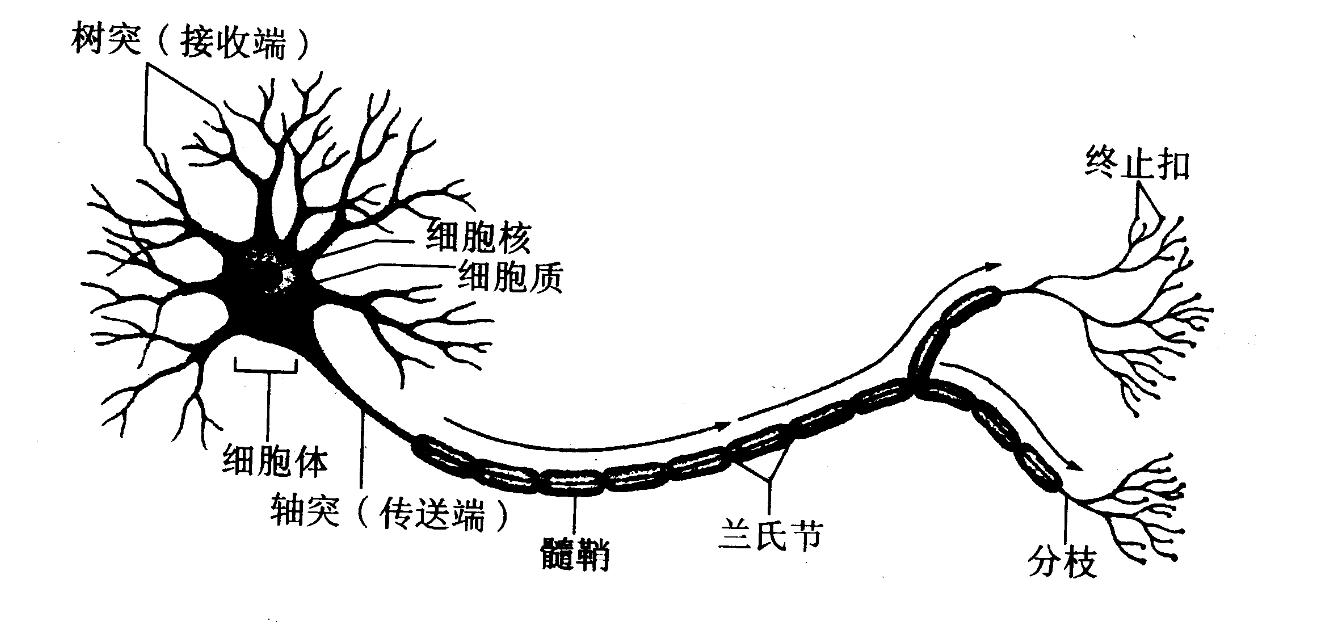
\includegraphics[height=6cm]{neuron}
  \caption{生物神经元的结构以及信息传递方式}
%  \label{fig:xfig1}
\end{figure}

%神经网络中的神经元可分为三个部分:输入信号、连接权重和激活函数。人脑皮层神经系统成为了人工神经网络出现的基础。人工神经网络的工作机制就是模仿生物神经元处理信息的机制,其中人工神经网络中的神经元相当于人脑神经系统中的神经元,通过激励和反馈,传递和处理信息。1943年,美国心理学家在总结了生物神经元基本特性的基础上,首先提出了神经元的数学模型,该模型很好地抽象了生物神经元的本质,并且忽略了复杂的生理学细节。该模型的提出,大大促进了人工神经网络的相关研究工作。


\subsection{人工神经网络概念}
人工神经网络就是由大量神经元组成多个网络层,将网络层相互连接组成的网络结构,其中多层前馈感知器就是其中最具代表性的一个模型。多层前馈感知网络是由2-3层网络层组成,对于相邻网络层中,上层网络层的神经元输出作为下层网络层的输入,同层内的神经元间相互独立没有连接。该网络结构保证输入信号从输入端开始传入,在网络中信号只是单方向地在网络处理与传递。

\begin{figure}[H] % use float package if you want it here
  \centering
  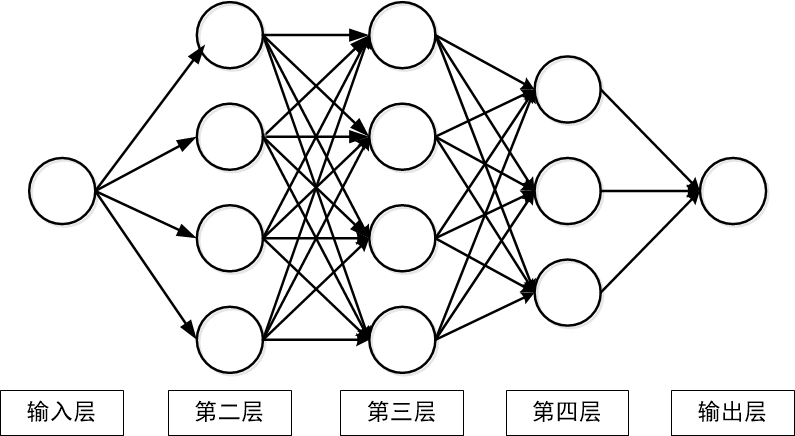
\includegraphics[height=6cm]{forward}
  \caption{人工神经网络的前馈网络}
  \label{fig:system}
\end{figure}


根据功能,根据多层前馈神经网络的信息处理方式和结构位置,其可以分为三个部分:第一部分是输入层,位于网络结构的起始段,作为输入信号进入网络结构的通道;第二部分是隐藏层,主要指在网络结构中由多个网络层的总称,其功能是实现数据的处理与计算功能;第三层是输出层,位于网络结构的终止端,用来输出前馈网络的计算结果。


神经元单元是神经网络系统中最重要的基础,一个神经元可简要地分为为三个部分:输入信号,连接权重和激活函数。神经元的工作机制可归纳为:处于抑制状态下的神经元,其树突接收到来自其他神经元所传递的兴奋激励信息,该激励信息可以由多个神经元所传递的信息组成;如果该激励信息超过某个限定值,那么接收信息的神经元则会由抑制状态转换为兴奋状态。


\begin{figure}[H] % use float package if you want it here
  \centering
  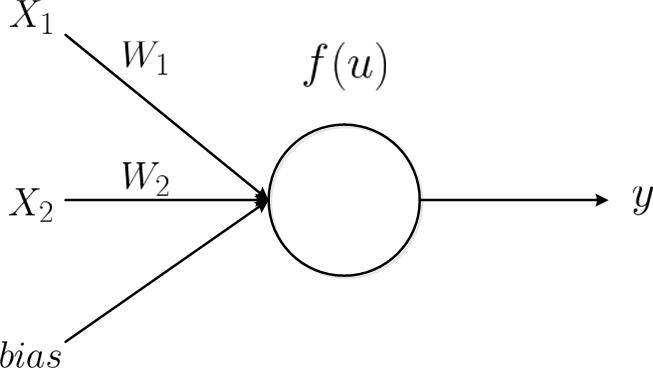
\includegraphics[height=4cm]{activation}
  \caption{人工神经网络中的神经元中信息传递过程}
  \label{fig:neuron}
\end{figure}


神经元的模型如图~\ref{fig:neuron}所示,该神经单元将接受的信息$X_1$,$X_2$,$\dots$,$X_n$,作为基础输入,这些输入就是原始输入信息或者上一个神经元所传递过来的信息;连接线条的数值$W_1$,$W_2$,$\dots$,$W_n$表示神经元之间具体的连接系数,即连接权值,表示轴突之间神经元的连接强度,通过点积的形式合输入相互结合,再加上一个偏置项对输入进行调整,通过激活函数$f(x)$进行判断,得到该神经单元最后的输出结果。激活函数通常是sigmoid函数和双曲正切函数,但是随着神经网络结构的不断地改进与复杂化,越来越多种形式的激活函数被应用到神经网络中。

图~\ref{fig:neuron}中的神经元模型具体的数据传递与激励计算过程可以表现为下列形式:
\begin{equation}
y=f(W_1 X_1 + W_2 X_2 + b)
\end{equation}

%人工神经网络系统就是大量的神经元互相连接而形成的复杂网络系统,即通过将多个网络层组装在一起形成一个复杂的网络系统,而相邻网络层之间就是用网络层内的神经元实现连接,多个神经元以权值表示连接强度实现连接,一个神经元的输出就是下一层的另一个神经元的输入,通过多个网络层的信息传递最终传输到输出层,得到网络的预测结果。
人工神经网络系统就是大量的神经元互相连接而形成的复杂网络系统,即通过将多个网络层组装在一起形成一个复杂的网络系统。根据单个神经元的数据处理过程,即可推导出在含有多个神经元的人工神经系统中,信息的具体传递方式。在如图~\ref{fig:system}的人工神经网络中,不同层神经元的信息传播可以表达为以下形式:
\begin{equation}
u_{j}^{(l)} = \sum_{i=1}^{n} W_{ij}^{(l-1)} X_{i}^{(l-1)} + b_{j}^{(l-1)}
\end{equation}
\begin{equation}
X_{j}^{(l)}=f(u_{j}^{(l)})
\end{equation}
其中,$W_{ij}^{(l-1)}$表示第$l-1$层中的第$i$个神经元输出对应第$l$层中的第$j$个神经元输入对应的连接权值。$X_i^{(l-1)}$表示第$l-1$层中的第$i$个神经元的输出,作为第$l$层的多个输入之一,$u_{j}^{(l)}$表示从$l-1$层的输出和对应权值的点积以及偏置项的加权和,作为$l$层第$j$个神经元的输入值。$f(x)$表示该神经元的激活函数。$X_{j}^{(l)}$表示$l$层的第$j$个神经元的输出,即传递到$l+1$层的多个输入之一。

输入信号在神经网络中经过网络隐含层的处理与传递后,逐层传播,最后在输出层得到神经网络的输出预测值。随后将预测值与实际值进行比较,设置损失函数,表示网络的性能,即对样本数据的拟合与表达能力。损失函数越小,则表示网络的预测值越符合真实情况,网络的性能越好;否则相反。根据具体要求不同,网络所采用的损失函数也是不一样的,比较常见的损失函数有:平方损失函数、指数损失函数、Hinge损失函数和log对数损失函数等。

\begin{equation}
h_{W,b}(X)=f(u^{(l)})
\end{equation}
\begin{equation}
E=\frac{1}{2m}\sum_{i=1}^{m}[h_{W,b}(X)_{i}-y_{i}]^{2}
\end{equation}
上述公式中的$h_{W,b}(X)$表示了网络的输出值,$y_{i}$表示了样本数据对应的实际值。假设这里的网络中使用了平方损失函数,则就要将预测值与实际值之间的差值进行平方处理,形式就如上述的损失计算公式。

如果根据图~\ref{fig:system}所示的话,而该网络的输出值和损失函数可表示为如下形式:
\begin{equation}
h_{W,b}(X)=f(u^{(5)})
\end{equation}
\begin{equation}
E=\frac{1}{2}(h_{W,b}(X)-y))^{2}
\end{equation}

\subsection{反向传播算法}

反向传播算法(Back-Propagation),也叫做误差反向传播或BP算法,常与最优化求解(如梯度下降法)相结合使用的,用来训练人工神经网络的经典方法。如果在训练过程中,使用了反向传播算法的网络,则也可称之为BP网络。BP算法的提出,使其成为了在监督学习的方式下训练多层前馈神经网络的典型且有效的方法,而且使神经网络开始具有广泛的应用潜力,也是目前最广为人知的人工神经网络模型之一。

BP算法是基于误差修正学习规则,使用梯度下降算法来最小化预测输出值与样本数据真实值之间的差值所构成的损失函数。BP算法实际上就是利用输出层的误差,来推导计算输出层上一层网络层神经元对应的误差数值,再利用所得到的误差数值继续推导计算更前层网络层相对应的误差值,以此类推,根据输出端预测误差逐级计算得到各层网络层的误差值,并且将这些梯度误差值沿着与输入信号传送相反的方向传递,则称之为反向传播算法。

BP网络主要是基于误差反向传播的多层前馈网络,但是早期的多层前馈神经网络只有信息的前向传播,BP网络提升了前馈网络的性能。与之前所使用的多层前馈网络相同,BP网络同样是由三个部分组成:输入层、隐含层和输出层;网络层之间的神经单元采用全连接方式传递数据,同层神经元之间独立无相互连接,这些特性都与之前提出的前馈神经网络相同。在BP网络结构中,输入层和输出层的神经元个数是由实际情况决定的,可以通过设置网络隐含层的层数以及每层中神经元节点的数目提升网络性能。

但是与之前所提出的前馈神经网络不同,BP网络最关键的地方通过误差信息的反向传播,调整网络中的权值,其学习的过程可以归纳为两部分:(1)输入信息的正向传播。在输入层传进数据信息作为输入信号,经过隐含层的数据处理和计算,最后在输出层输出预测结果值;信号在网络传递的过程中,网络中的连接权值是恒定不变的,每一层神经元的状态只会对下一层神经元的状态产生作用,对其他网络层没有影响。而网络中的每一层的权值是在反向传播过程中,通过对实际结果与预测结果的误差,对网络中的各层的权值进行调整,使网络最终的预测值更靠近实际结果。(2)误差信息反向传播:网络输出的预测结果值与样本数据的真实值比较的差值,即为误差信号。误差信息由输出端开始逐层沿着与输出信号传递相反方向进行传播,直到网络的输入端。输入信号的传递为前向传播,逐层朝正向方向递进传播;而误差信号的传递是沿相反方向实现传递,则为反向传播。在误差信号的反向传播过程中,网络的权值根据误差值的大小,不断改进网络的连接权值,通过迭代式地对连接权值进行修改,提升网络性能,使网络的输出预测值更接近实际样本的真实值。

\begin{figure}[H] % use float package if you want it here
  \centering
  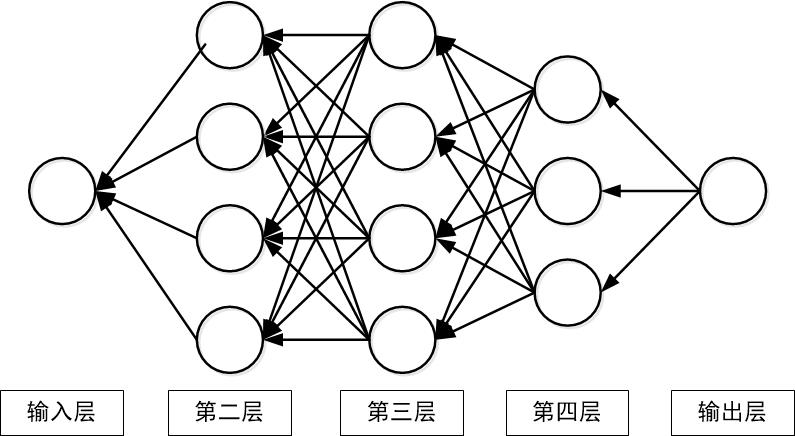
\includegraphics[height=6cm]{bp}
  \caption{人工神经网络中的误差反向传递的过程}
  \label{fig:bp}
\end{figure}

如图~\ref{fig:bp}中所示的在神经网络误差信息反向传播,该网络最终的输出可以表达为:
\begin{equation}
h_{W,b}(X)=f(u^{(5)})
\end{equation}

在这个网络中,损失函数通过log对数的形式表达,该方式如下:
\begin{equation}
J(W,b)=E=-\frac{1}{m}[\sum_{i=1}^{m} y_{i} log(h_{W,b}(X)_{i}) +
		(1-y_{i})log(1-h_{W,b}(X)_{i})]
\end{equation}
其中$h_{W,b}(X)_{i}$表示神经网络输出层的第$i$个输出单元的输出值,$y_{i}$表示样本数据中对应的第$i$个实际值,$J(W,b)$是根据网络输出层误差所计算的损失函数$E$的另一种形式。

由于反向传播算法传播的主要是每一层的相对误差信息,并且通过比较图~\ref{fig:system}和图~\ref{fig:bp}可以看出,误差信息的传播方向和输入信息的传播方向恰恰相反,在这里输入端的误差作为输入信号,在网络中进行传播。因此,首先需要计算输入层的误差,其表达形式如下:
\begin{equation}
\delta_{j}^{(5)}=h_{W,b}(X)_{j}-y_{j}
\end{equation}
在网络的反向传播中,都使用$\delta$表示所传递的误差值,则$\delta_{i}^{(5)}$表示第$5$层输出层中第$i$个神经元的误差值。

而对于之前的隐含层的误差计算,由于激励函数的存在,因此误差在经过激励函数时,需要对激励函数进行求导计算,因此,误差信息在隐含层的表示如下:
\begin{equation}
\delta_{i}^{(l-1)}=(\sum_{j=1}^{m} W_{ji}^{(l-1)} \delta_{j}^{(l)}) f'(u_{i}^{(l-1)})
\end{equation}

其中$\delta_{i}^{(l-1)}$表示$l-1$层中第$i$个神经元所计算的误差值,$W_{ji}^{(l)}$是第$l$层的第$i$个神经元对应第$l-1$层的第$j$个神经元的连接权值,为前向传播所对应的$W_{ij}^{(l)}$的转置形式,$\delta_{j}^{(l)}$表示$l$层中第$j$个神经元所计算得到的误差值。$f'(u_{j}^{(l-1)})$表示对$l-1$层的激励函数求导所得到的结果。

BP算法主要是根据梯度下降的方向,对问题进行求解,得到全局最小值作为最优解。在神经网络中,需要对网络层之间的连接权值$W_{ij}^{(l)}$和$b^{l}$进行更新,因此需要通过对损失损失函数用权值求偏导,求解最小梯度最小方向。
\begin{align}
\frac{\partial J(W,b)}{\partial W_{ij}^{(l)}} & = {\frac{\partial J(W,b)}{\partial u_{i}^{(l+1)}}} {\frac{\partial u_{i}^{(l+1)}}{\partial W_{ij}^{(l)}}}  \\
					    & =  X_{j}^{(l)} \delta_{i}^{(l+1)} \\
\frac{\partial J(W,b)}{\partial b_{i}^{(l)}} & = \frac{\partial J(W,b)}{\partial u_{i}^{(l+1)}} {\frac{\partial u_{i}^{(l+1)}}{\partial b_{i}^{(l)}}} \\
					    & = \delta_{i}^{(l+1)}
\end{align}

由以上公式,可以得到网络中每层对应的权值和偏置项的梯度方向,根据梯度下降法,则可以对权值$W_{ij}^{(l)}$和偏置项$b_{i}^{(l)}$进行更新:
\begin{align}
W_{ij}^{(l)} & = W_{ij}^{(l)} - \alpha \frac{\partial J(W,b)}{\partial W_{ij}^{(l)}}  \\
	     & = W_{ij}^{(l)} - \alpha X_{j}^{(l)} \delta_{i}^{(l+1)} \\
b_{i}^{(l)} & = b_{i}^{(l)} - \alpha \frac{\partial J(W,b)}{\partial b_{i}^{(l)}} \\
	    & = b_{i}^{(l)} - \alpha \delta_{i}^{(l+1)}
\end{align}
其中,$\alpha$表示网络初始设置的学习率。学习率为较大的值,可以使网络更快收敛,但是也可能造成网络得到局部最优解,甚至训练到一定程度后造成无法收敛的情况,因此学习率的设置也是非常重要的。

以上的计算实现了反向传播算法一次迭代的过程,但是在反向传播中需要实现多次迭代得到最优解,这里用$\bigtriangledown_{W^(l)} J(W,b)$表示$J(W,b)$对$W^{(l)}$的偏导,用$\bigtriangledown_{b^(l)} J(W,b)$表示$J(W,b)$对$b^{(l)}$的偏导。则反向传播算法的具体步骤可以表示为:
\begin{enumerate}
\item 初始化:对网络中所有层的权值$W_{ij}^{(l)}$和偏置项$b^(l)$进行初始化。
\item 进行前向传播,在网络计算输出值,以及损失函数值$J(W,b)$。
\item 进行反向传播,计算梯度$\bigtriangledown_{W^(l)} J(W,b)$和$\bigtriangledown_{b^(l)} J(W,b)$。
\item 更新各层的权值$W^{(l)}$和偏置项$b^{(l)}$,更新后逐步减小损失函数$J(W,b)$。
\item 判断是否达到迭代次数,如果达到次数,则进行下一步;如果没有达到次数,则返回第二步。
\item 根据网络输出,得到最终结果。
\end{enumerate}


%%%%%%%%%%%%%%%%%%%%%%%%%%%%%%%%%%%%%%%%%%%%%%%%%%%%%%%%%%%%%%%%%%%%%%%%%%%%%%%
\section{卷积神经网络}

\subsection{卷积神经网络发展历程}
卷积神经网络最初是受到生物神经学信息处理原理和机制的启发,成为人工神经网络众多网络模型中,流传最广、最常使用的网络之一。相对于普通特征提取方法而言,更强的适用性、特征提取能力、学习能力强和训练参数少是卷积神经网络最主要的特点。另外,卷积神经网络的泛化能力强等优点,使其成为图像识别相关领域非常重要的研究热点。

1962年,通过研究猫观察事物时,其神经的视觉皮层细胞的活跃情况,Hubel和Wiesel提出了感受野概念\cite{hubel1968receptive}。在人类的视觉神经系统中,人脑的输入神经信号是由眼睛上的视网膜光感受器接受光和场景信息所转换而成的。当感受器受刺激兴奋时,感受器官中的神经元会将外界的视觉信息以刺激信号的形式传递人脑更高级的神经细胞中,其中神经元用来对视觉信息产生刺激信号的区域就叫做神经元的感受野。

随后,感知机概念的提出是由Fukushima在20世纪80年代提出的\cite{fukushima1980neocognitron},其可以被认为是深度学习的起源,也可以视为卷积神经网络最初的表示形式,同时也是感受野相关概念首次实际应用于人工神经网络领域的。感知机与卷积神经网络不同的地方在于它没有使不同位置的神经元共享一个训练得到的权值;但是,感知机将所接收的视觉信息分解成多个较小模块化形式的低层次子特征,然后在这些低层次字特征通过多层次的特征平面化计算与处理,在区域平面化理的基础上,使用较少的计算量和参数量就能实现对输入数据的训练与传递,实现相应的识别。感知机是一个典型的多层神经网络模型,其中隐含层中的局部区域信息与局部感受野激发后生成了下一层的响应值。这种局部区域感受野的信息处理机制,可以避免信息处理过程中区域位置、大小和尺度的影响。另外,感知机采用的无监督学习也是卷积神经网络早期研究中占据主导地位的训练方式。 

1989年,LeCun在神经网络中的反向传播加入了一些限制,用来增强网络的学习能力,提高网络最终的预测能力\cite{lecun1998gradient}。他在训练 LeNet-5 网络的过程中使用了基于梯度下降方向传播算法,保证网络能够有监督学习与训练。手写数字图像在LeNet-5中多个卷积层、下采样层和全连接层的训练与作用下,图像转换为大量特征映射图,这些特征映射图就包含了高层次、抽象的辨别特征。卷积层中卷积核的作用相当于感知机中的区域感受野,通过卷积核的卷积处理,将图像中各个区域的局部信息提取为更具体、更有效、维度更小的特征信息。1998年,在手写数字体数据的识别中,使用深度学习技术的 LeNet-5 网络所取得的准确率超过了之前特征提取等方法的结果,而如今所流行的卷积神经网络模型都是沿用 LeNet-5 的卷积层、池化层和全连接层结构为模板而设计的。 

随后在2012年,卷积神经网络被Krizhevsky\cite{krizhevsky2012imagenet}等人应用在当年ImageNet的ILSVRC比赛,他们提出了名为AlexNet的卷积网络模型,并且赢得了比赛中图像分类和物体检测的双项第一名,在图像分类中领先第二名大约11\%的准确率,以极大优势获胜,这也是卷积神经网络在大规模自然图像数据中第一次的实际应用,实现了卷积神经网络性能的进一步提高,为深度学习在如今生活方方面面的应用拉开序幕。随后,不断有新的卷积神经网络模型被提出,比如牛津的VGGNet\cite{simonyan2014very},谷歌的GoogLeNet\cite{szegedy2015going},微软的ResNet\cite{he2015deep}等,这些网络模型不仅在ImageNet数据集上刷新着识别率记录,并且在其他许多数据集上也取得了最优异的结果,因此卷积神经网络在当前图像识别相关领域起着非常重要的作用。

由于基于卷积神经网络的深度学习结构具有非常强大的学习与表达能力,因此卷积神经网络不仅被应用在图像识别领域,而且也在视频分析和自然语言处理等方面具有很大的应用潜力,取得了非常好的成果。

%%%%%%%%%%%%%%%%%%%%%%%%%%%%%%%%%%%%%%%%%%%%%%%%%%%%%%%%%%%%%%%%%%%%%%%%%%%%%%%%%%%%%
\subsection{卷积神经网络原理和组成}

卷积神经网络最关键的部分为卷积核,卷积核与输入图像或者中间层的特征映射的不同小区域相连,通过卷积核的卷积处理,将图像信息具体化和转换,获取高层次特征信息。典型的卷积神经网络是由3种不同的神经层组成:卷积层,池化层和全连接层。传统的卷积神经网络是将卷积层和池化层进行组合连接的,以此来减少计算时间、逐步构建和提取更深层次的空间不变性。随后通过全连接层的特征转换,即可得到网络最终的输出。下面将主要介绍这个些结构单元的作用:

\begin{enumerate}
\item 卷积层

卷积层作为典型的深度神经网络,卷积神经网络中卷积层的每一个神经元是由前向传输层的局部感知域和所学习到的卷积核权值作为输入所组成的。在同一个特征映射图的神经元共享同样的卷积核,但是这个被共享的卷积核是用不同的输入感知域所得到的。在同一个卷积层中,由不同的特征映射所得到的卷积核是不同的。经过研究,卷积核的大小和数量表示了网络的宽度,网络宽度会对网络的性能造成影响。

实际上,在卷积层中,信息的前向传播主要是由上一层的特征映射和该层中可学习参数的卷积核进行卷积计算,再加上卷积层的偏置项的调整,经过激活函数进行计算处理的,就会得到该层每个卷积核所对应的输出特征映射。卷积层的卷积计算可以表达为以下公式:
\begin{equation}
X_{j}^{(l)} = f(\sum_{i} X_{i}^{(l-1)}  K_{ij}^{(l)} + b_{j}^{(l)})
\end{equation}
$X_{j}^{(l)}$表示第$l$层的卷积层的第$j$个输出特征映射;$X_{i}^{(l-1)}$表示第$l-1$层的第$i$个输出特征映射,即第$l$层的卷积层的输入;$K_{ij}^{(l)}$表示第$l$层中处理第$i$个输入特征映射到第$j$个输出特征映射所对于那个的卷积核;$b_{j}^{(l)}$是在第$l$层的第$j$个特征映射所对应的偏置项。在第$l$个卷积层的不同输出特征映射尽管是由相同的输入特征映射得到的,但是不同的输出特征映射所对应的卷积核是不同的。

\begin{figure}[H] % use float package if you want it here
  \centering
  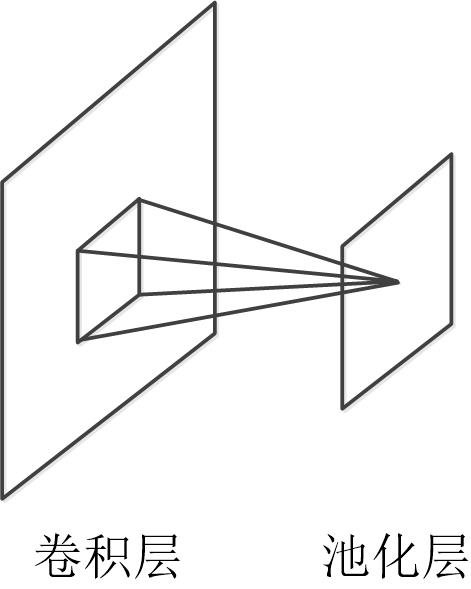
\includegraphics[height=5cm]{convolution}
  \caption{卷积神经网络中卷积层的信息处理}
\end{figure}


\item 池化层 

池化层是非线性下采样的一种形式,它的功能是不断减少表示特征的特征映射图的空间尺寸,用来达到减少参数数量和降低网络计算量的目的,另外也能实现控制过拟合的问题。而且,它也提供了平移不变性。池化层只是改变了输入映射图的尺寸,但是不改变输入映射的数量。平均池化和最大值池化是池化层比较常用的操作,其中最大值池化是最常用的操作,并且也应用在后续的实验当中。
\begin{equation}
X_{j}^{(l)} = f( \beta_{j}^{(l)} down(X_{j}^{(l-1)}) + b_{j}^{(l)})
\end{equation}			
其中$X_{j}^{(l)}$表示第$l$层的池化层的第$j$个输出特征映射;$\beta$是常量,用来控制池化层对数据的调整;$down(\cdot)$表示下采样处理,形式可能就是最大池化或者平均池化;$b_{j}^{(l)}$表示第$l$层的池化层中对第$j$个输出特征映射偏置的调整。因为池化层不改变特征映射数量,因此在这里经过池化处理,特征映射个数仍保持不变。

\begin{figure}[H] % use float package if you want it here
  \centering
  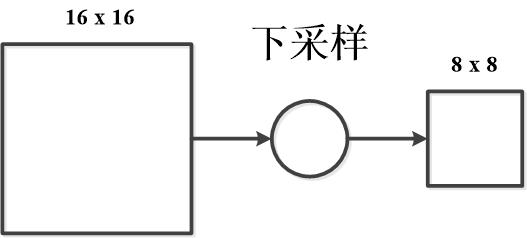
\includegraphics[height=3cm]{pooling}
  \caption{卷积神经网络中池化层的信息处理}
\end{figure}

\item 全连接层

全连接层的表示方式,就如常规的神经网络一样,全连接层中的神经元以全连接的形式进行数据的计算和信息的传递。因此,全连接层的激活函数可以通过矩阵乘法与偏差值计算来表示:
\begin{equation}
X_{j}^{(l)}=f(u_{j}^{(l)})=f(\sum_{i=1}^{m} W_{ij}^{l-1} X_{i}^{(l-1)} + b_{j}^{(l-1)})
\end{equation}
$X_{j}^{(l)}$是第$l$层为全连接层的第$j$个神经元的输出值;$W_{ij}^{l}$是第$l-1$层的第$i$个神经元到第$l$层的第$j$个神经元的连接权值;$X_{i}^{(l-1)}$是第$(l-1)$层中第$i$个神经元的输出值,$b_{j}^{(l-1)}$表示第$l-1$层对第$j$个输出特征映射的偏置,$f(x)$为激活函数。全连接层的计算方式与普通人工神经网络的传递方式基本相同,而且也是卷积神经网络中占据大量的参数和计算量的部分。

\end{enumerate}


%%%%%%%%%%%%%%%%%%%%%%%%%%%%%%%%%%%%%%%%%%%%%%%%%%%%%%%%%%%%%%%%%%%%%%%%%%%%%%%%%%%%%%%
\subsection{卷积神经网络的反向传播}

卷积神经网络的反向传播算法与普通人工神经网络的反向传播算法相同,也是将误差进行反向传播,同时根据梯度下降法,对网络中的参数进行调整与更新。卷积层、池化层和全连接层是卷积神经网络的基础部分,在卷积层和池化层中的信息处理和传递与普通前向传播方法不同,由于卷积层和池化层中传输的为特征映射,因此卷积神经网络的误差主要也是以特征映射的形式进行反向传播的,可称之为特征映射误差。对于全连接层,其前向传播和后向传播与普通神经网络相同,计算方式已在之前章节提到。所以接下来主要介绍卷积层和池化层的信息反向传播。 

\begin{enumerate}
\item 卷积层

假设目前第$l$层为卷积层,后面一层第$l+1$层为池化层,根据反向传播算法可知,为了要计算第$l$层的误差,我们需要知道$l+1$层的误差以及该层神经元所传递的输入加权和$u^{(l)}$。对于从卷积层到池化层的信息传递,实际上是卷积层一块像素组成的输出特征映射,变换为池化层的一个像素;因此,池化层中某点的误差,就对应了卷积层中某块像素对应的特征映射的误差值。为了保证有效计算出第$l$层卷积层中误差,将第$l+1$层池化层中的误差进行上采样处理,使其具有和卷积层的映射具有相同的尺寸,然后再将上采样的误差与$l$层的激活函数导数进行点乘即可。
\begin{equation}
\delta_{j}^{(l)} = \beta_{j}^{(l+1)} ( f'(u_{j}^{(l)}) * up(\delta_{j}^{(l+1)}))
\end{equation}
其中,$up(\cdot)$表示上采样处理,只是将输出的像素在水平方向和竖直方向拓展一定的倍速,形成一块像素区域,区域中每个像素值都相同;$\delta_{j}^{(l)}$表示第$l$层卷积层第$j$个特征映射对应的误差,$\beta_{j}^{(l+1)}$是第$l+1$层池化层中的常量,表示对误差进行相应的运算;$f'(u_{j}^{(l)})$表示激活函数的导数。

在计算出特征映射误差的前提下,通过对所有误差求和即可得到偏置项的梯度,其中$(u,v)$表示输出特征映射像素点的位置:
\begin{equation}
\frac{\partial E}{\partial b_{j}^{(l)}} = \sum_{u,v} (\delta_{j}^{(l)})_{uv}
\end{equation}

而对于网络层中卷积核的权值也可以用所得的误差计算得出:
\begin{align}
\frac{\partial E}{\partial K_{ij}^{(l)}} & = \sum_{u,v} (\delta_{j}^{(l)})_{uv} (p_{i}^{(l-1})_{uv} \\
					 & = rot180(conv2(X_{i}^{(l-1)}, rot180(\delta_{j}^{(l)})))
\end{align}
其中$(p_{i}^{(l-1})_{uv}$是$X_{i}^{(l-1)}$中与$K_{ij}^{(l)}$进行卷积计算的像素块,为了计算得到输出特征映射$X_{j}^{(l)}$中在位置$(u,v)$的像素;$rot180(\cdot)$表示对矩阵进行旋转180度处理;$conv2(\cdot)$表示卷积运算。

在求得卷积核偏导数和偏置项的偏导数后,即得到卷积核参数和偏置项的梯度方向,即可更具下列公式对卷积神经网络的参数进行更新:
\begin{align}
K_{ij}^{(l)} & = K_{ij}^{(l)} - \bigtriangledown_{K_{ij}^{(l)}} E \\
b_{j}^{(l)} & = b_{j}^{(l)} - \bigtriangledown_{b_{j}^{(l)}} E 
\end{align}
\item 池化层

假设目前第$l$层为池化层,后面一层第$l+1$层为卷积层,这种情况与之前的完全相反。但是同样,首先需要算出第$l+1$层的误差值。如果计算出了误差值后,则只需要对参数$b$进行更新即可。如果池化层后紧随的是全连接层,那么采样层的误差则可根据普通神经网络的反向传播算法进行计算。

一般情况下,如果池化层如果没有偏置项,则池化层不需要进行权值更新,但是仍然需要计算特征映射误差。当要计算卷积层中卷积核的梯度时,必须确定卷积层中输入特征映射中像素块所对应的输出特征映射的像素值。然而,在池化层必须确定特征映射误差的像素块对应下一层特征映射误差的像素值。则池化层的特征映射误差可以表示为:
\begin{equation}
\delta_{j}^{(l)}=f'(u_{j}^{(l)}) * conv2(\delta_{j}^{(l+1)}, rot180(K_{j}^{(l+1)})
\end{equation}
其中$\delta_{j}^{(l)}$表示第$l$层为池化层的第$j$个特征映射误差;$f'(u_{j}^{(l)})$表示激活函数的导数;同样,$rot180(\cdot)$表示对矩阵进行旋转180度处理;$conv2(\cdot)$表示卷积运算。
\begin{align}
\frac{\partial E}{\partial b_{j}^{(l)}} & = \sum_{u,v} (\delta_{j}^{(l)})_{uv} \\
b_{j}^{(l)} & = b_{j}^{(l)} - \bigtriangledown_{b_{j}^{(l)}} E 
\end{align}
对于池化层的偏置项求导与卷积层的偏置求导方法相同。同样,池化层的偏置项参数更新也与卷积层相同。

\end{enumerate}

%%%%%%%%%%%%%%%%%%%%%%%%%%%%%%%%%%%%%%%%%%%%%%%%%%%%%%%%%%%%%%%%%%%%%%%%%%%%%%%%%%%%%%%
\subsection{卷积神经网络模型}

\begin{enumerate}
\item LeNet-5\cite{lecun1998gradient}

LeNet-5是一个用来识别手写数字体图像的卷积神经网络,也是第一个可以实际应用于工业界的卷积神经网络,如今所提出的卷积网络模型都是参考了LeNet-5的模型所设计的。LeNet-5网络模型同样采用前向传播和后向传播的方法进行训练,但是由于每个网络层内部的权值共享,因此在保证了LeNet-5学习能力的前提下,大大减少了训练参数,加快了训练速度。LeNet-5网络模型不包括输入层,总共有7层网络层,每一层都包括可训练的权值参数,采用了交替连接的卷积层和下采样层对输入图像进行前向传导,并且最终通过全连接层输出概率分布的结构,LeNet-5网络模型如图~\ref{fig:lenet}所示。

\begin{figure}[H] % use float package if you want it here
  \centering
  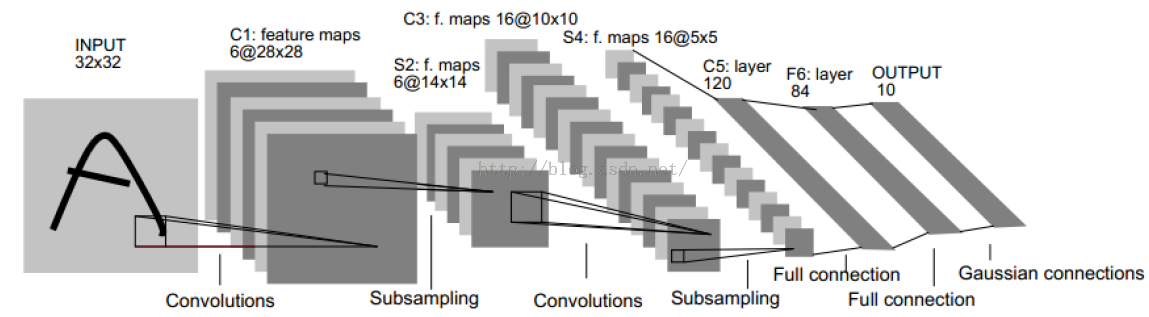
\includegraphics[height=3.5cm]{lenet}
  \caption{LeNet-5卷积神经网络模型}
  \label{fig:lenet}
\end{figure}


\item AlexNet\cite{krizhevsky2012imagenet}

在2012年的图像大规模视觉识别挑战赛 (ImageNet Large Scale Visual Recognition Challenge, ILSVRC)上,基于卷积神经网络的AlexNet横空出世,在图像分类和物体检测中都取得了双项冠军,在图像分类竞赛中相比于第二名在准确率上取得了高出11\%的优势,使得卷积神经网络的研究从此引起了学术界的高度关注,也开启了深度学习在各个领域应用的大门。AlexNet有5层卷积层,以及3层全连接层,约65万个神经元以及6000万个可训练参数,从网络规模上大大超越了LeNet-5。AlexNet使用了修正线性单元(Rectified Linear Units,ReLU)作为激活函数,取代了传统的sigmoid函数或tanh函数。而使用修正线性单元的网络训练速度将比使用tanh函数的网络快了将近六倍左右。局部响应归一化(Local Response Normalization,LRN)在训练过程中对所有输入信息进行归一化处理,保证邻近抑制,促进了训练速度。另外,深度网络经常会在训练过程中产生过拟合问题,造成网络性能下降,而基于dropout的技术,从一定程度上减轻了网络过拟合问题,提升了网络的准确率。另外,AlexNet还使用了多显卡进行网络的训练,与传统的处理器运算相比,显卡的逻辑运算功能大大强于处理器,在训练速度上提高了十多倍以上。AlexNet网络模型如图~\ref{fig:alexnet}所示。
%AlexNet满足了深度学习最基本的三个要求:大量的训练数据,合理的网络结构和强大的学习能力。

\begin{figure}[H] % use float package if you want it here
  \centering
  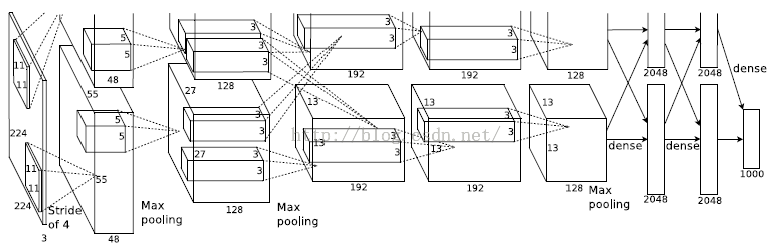
\includegraphics[height=4cm]{alexnet}
  \caption{AlexNet卷积神经网络模型}
  \label{fig:alexnet}
\end{figure}

\item GoogLeNet\cite{szegedy2015going}

Google公司在2014年的图像大规模视觉识别挑战赛 (ImageNet Large Scale Visual Recognition Challenge, ILSVRC)上,提出了GoogLeNet卷积神经网络模型。GooLeNet是一个具有22层网络层的深度卷积神经网络,这个模型最主要的特点就是提出了Inception单元,大幅度提高了网络计算资源的非线性能力。Inception是一个人工设计实现的非线性计算单元,在保持计算损耗不变的前提下,提升了网络的深度与宽度,以此来提高了网络的计算能力与非线性的表达能力。为了提高求解能力,GooLeNet还采用了Hebbian准则和多尺度处理方法来提高决策能力。GoogLeNet主要从两个方面提高网络模型的学习能力:网络的深度(网络层数)和网络的宽度(卷积核数量),但是相对产生的问题就是网络太深,梯度可能会消失,难以训练;参数太多,容易造成过拟合;以及网络计算复杂度太大,难以应用。为了解决以上问题,GoogLeNet从两个方面进行解决:(1)深度上,GoogLeNet为了避免梯度消失问题,在不同深度的位置增加了两个损失函数保证梯度顺利地回传;(2)宽度上,将多尺度的卷积核和池化处理组合成一个Inception单元结构,不仅可以减少网络参数,降低网络计算复杂度,而且很好地提升了网络的非线性表达能力。同时,Inception单元结构也是GoogLeNet最突出的特点,其具体结构如图~\ref{fig:inception}所示。

\begin{figure}[H] % use float package if you want it here
  \centering
  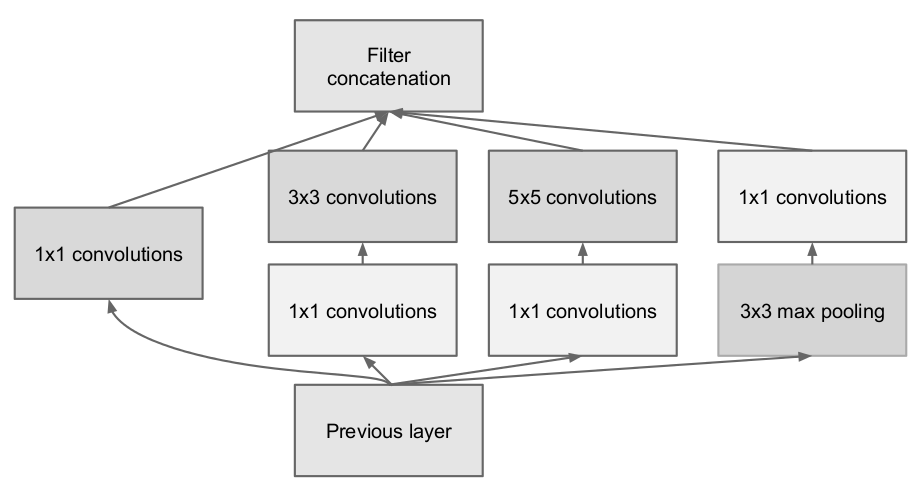
\includegraphics[height=4.5cm]{inception}
  \caption{GoogLeNet网络模型中的Inception单元结构}
  \label{fig:inception}
\end{figure}

\end{enumerate}



\section{本章总结}
本章主要介绍了深度学习的相关概念,人工神经网络中的生物神经基础、基本知识和反向传播算法,以及卷积神经网络的原理、机制和模型。深度学习是机器学习领域一个新的研究方向,以大量的样本数据为基础,在具有深层次的网络结构的条件下,通过庞大的计算量以及有效的训练方法使网络学习和表达数据中潜在的规律,实现网络对数据的拟合与预测。因此,人工神经网络是深度学习的基础,而人工神经网络是收到生物神经系统的启发而研究的,其目的在于模拟人脑中对于信息的处理方式来处理和分析大量的数据。人工神经网络具有前向传播和后向传播两种方式,其中后向传播算法是保证网络能够得到有效训练,更符合数据规律的关键。

卷积神经网络是深度学习中一个经典、应用最广泛的算法之一,目前已经在图像识别、视频分析、自然语言处理等各个领域取得了非常显著的成绩。卷积神经网络主要是由卷积层、池化层和全连接层组成,其从样本数据出发,隐式地从训练数据中学习规律;由于局部权值共享的特点,很大程度减少了需要训练参数数量,大大降低了网络复杂性,提取和转换平移、尺度和其他形式的扭曲不变形特征,具有非常好的效果。









